\documentclass[10pt]{article}
\setlength{\oddsidemargin}{0.25 in}
\setlength{\evensidemargin}{-0.25 in}
\setlength{\topmargin}{-0.6 in}
\setlength{\textwidth}{6.5 in}
\setlength{\textheight}{8.5 in}
\setlength{\headsep}{0.75 in}
\setlength{\parindent}{0 in}
\setlength{\parskip}{0.1 in}

\usepackage{graphicx}
\usepackage{url}

\usepackage{float}
\usepackage{hyperref}

%
% The following commands sets up the lecnum (lecture number)
% counter and make various numbering schemes work relative
% to the lecture number.
%
\newcounter{lecnum}
\renewcommand{\thepage}{\thelecnum-\arabic{page}}
%\renewcommand{\thesection}{\thelecnum.\arabic{section}}
\setcounter{section}{15}
\renewcommand{\theequation}{\thelecnum.\arabic{equation}}
%\renewcommand{\thefigure}{\thelecnum.\arabic{figure}}
\renewcommand{\thetable}{\thelecnum.\arabic{table}}
\newcommand{\dnl}{\mbox{}\par}

%
% The following macro is used to generate the header.
%
\newcommand{\lecture}[4]{
  \pagestyle{myheadings}
  \thispagestyle{plain}
  \newpage
  \setcounter{lecnum}{#1}
  \setcounter{page}{1}
  \noindent
  \begin{center}
  \framebox{
     \vbox{\vspace{2mm}
   \hbox to 6.28in { {\bf CMPSCI~630~~~Systems
                       \hfill Spring 2023} }
      \vspace{4mm}
      \hbox to 6.28in { {\Large \hfill Lecture #1  \hfill} }
%       \hbox to 6.28in { {\Large \hfill Lecture #1: #2  \hfill} }
      \vspace{2mm}
      \hbox to 6.28in { {\it Lecturer: #3 \hfill Scribe: #4} }
     \vspace{2mm}}
  }
  \end{center}
  \markboth{Lecture #1: #2}{Lecture #1: #2}
  \vspace*{4mm}
}

%
% Convention for citations is authors' initials followed by the year.
% For example, to cite a paper by Leighton and Maggs you would type
% \cite{LM89}, and to cite a paper by Strassen you would type \cite{S69}.
% (To avoid bibliography problems, for now we redefine the \cite command.)
%
\renewcommand{\cite}[1]{[#1]}

% \input{epsf}

%Use this command for a figure; it puts a figure in wherever you want it.
%usage: \fig{NUMBER}{FIGURE-SIZE}{CAPTION}{FILENAME}
%\newcommand{\fig}[4]{
%           \vspace{0.2 in}
%           \setlength{\epsfxsize}{#2}
%           \centerline{\epsfbox{#4}}
%           \begin{center}
%           Figure \thelecnum.#1:~#3
%           \end{center}
%   }

% Use these for theorems, lemmas, proofs, etc.
\newtheorem{theorem}{Theorem}[lecnum]
\newtheorem{lemma}[theorem]{Lemma}
\newtheorem{proposition}[theorem]{Proposition}
\newtheorem{claim}[theorem]{Claim}
\newtheorem{corollary}[theorem]{Corollary}
\newtheorem{definition}[theorem]{Definition}
\newenvironment{proof}{{\bf Proof:}}{\hfill\rule{2mm}{2mm}}

% Some useful equation alignment commands, borrowed from TeX
\makeatletter
\def\eqalign#1{\,\vcenter{\openup\jot\m@th
 \ialign{\strut\hfil$\displaystyle{##}$&$\displaystyle{{}##}$\hfil
     \crcr#1\crcr}}\,}
\def\eqalignno#1{\displ@y \tabskip\@centering
 \halign to\displaywidth{\hfil$\displaystyle{##}$\tabskip\z@skip
   &$\displaystyle{{}##}$\hfil\tabskip\@centering
   &\llap{$##$}\tabskip\z@skip\crcr
   #1\crcr}}
\def\leqalignno#1{\displ@y \tabskip\@centering
 \halign to\displaywidth{\hfil$\displaystyle{##}$\tabskip\z@skip
   &$\displaystyle{{}##}$\hfil\tabskip\@centering
   &\kern-\displaywidth\rlap{$##$}\tabskip\displaywidth\crcr
   #1\crcr}}
\makeatother

% **** IF YOU WANT TO DEFINE ADDITIONAL MACROS FOR YOURSELF, PUT THEM HERE:



% Some general latex examples and examples making use of the
% macros follow.

\begin{document}

%\lecture{**LECTURE-NUMBER**}{**DATE**}{**LECTURER**}{**SCRIBE**}
\lecture{16}{May 4}{Emery Berger}{Victor L.}

\section{Performance Analysis}
In this lecture, we discussed the measures and importance of performance in software, followed by dynamic analysis tools for performance profiling. In particular, prof, gprof, and Coz are discussed.

\subsection{What is "fast enough"?}
\href{https://www.modular.com/mojo}{Mojo} is a programming language developed by \href{https://www.nondot.org/sabre/}{Chris Lattner}. 
Lattner is also the creator of \href{https://llvm.org}{LLVM}, the now universal compiler for C/C++, and \href{https://www.swift.org}{Swift}, Apple's chosen language for application development on iOS.
In essence, Mojo is a dialect of the Python programming language that can be compiled down into C for the purposes of increased performance.

We obviously care a lot about speed, but how fast is fast enough? 
There are two primary measures of performance for computers: latency and throughput. 
Throughput is measured in transactions per second. 
Latency is measured as the time it takes from start to finish, and is useful for measurements such as latency of a transaction, update, or loading. 
There are some applications where having low latency is extremely important, such as high frequency trading (HFT), video games, and virtual reality (VR).
In HFT, having higher latency can result in huge monetary losses so many firms often install direct lines from their company servers to the trading servers on Wall Street.
With VR, having low latency is important not just for user experience, but having latencies that are not sufficiently low can result in motion sickness.
P99 latency is the 99th latency percentile, meaning that all requests are handled within a particular latency 99\% of the time.
This one percent is known as the tail latency, and it is often noticeable by users. 
A potential cause of users experiencing tail latency is running into a \href{https://en.wikipedia.org/wiki/Barrier_(computer_science)}{barrier computation}.
Barrier computations are computations that rely on a result from a previous step and cannot continue until that result has been resolved.

Other measures of performance include asymptotic analysis (Big O).
Due to the removal of constants, this is not always the best measure as $O(n) == O(1,000,000~n)$. 
Another example is standard matrix multiplication, which runs in $O(n^{3})$ time. 
\href{https://en.wikipedia.org/wiki/Strassen_algorithm}{Strassen's algorithm} can run in $O(n^{lg(7)}) == O(n^{2.807})$ which at first glance appears that it is faster.
However, there are a multitude of reasons why this is not so.
Firstly, on an elementary computer, Strassen's algorithm only offers a performance benefit for sufficiently large $n$.
Secondly, modern day computers with hardware vectorization can perform matrix multiplication using the naive algorithm faster.
Therefore, although asymptotically faster, Strassen's algorithm is not practical for real world applications.
It is noted that any algorithms that are $O(n^{2})$ or slower are not scalable.\\


\subsection{Performance Profilers}
The first performance profiler was \texttt{prof}, which was included in Unix. 
\texttt{prof} analyzed the program through it's executions, which we call dynamic analysis. The most basic way to profile a program to determine where to optimize it is by counting the number of executions of each line of code. 
However, this is not realistic as it assumes all lines of code take an equal amount of time to execute. 
For example, a line of code assigning a variable (e.g. \texttt{a = 3}) may execute 10x more than a more complex one (e.g. \texttt{a = sqrt($\pi^{30}$})), but it does not mean the first line requires more optimizing.

There are two common problems with performance profilers. 
First is that performing the recommended optimizations may not yield any performance improvements. 
Second is that the instrumentation used by these profilers often slow down the program it is profiling. 

One might think that a better approach than counting number of times lines are executed are to time the amount of time each line spends executing. 
However, there is a shortcoming related to the timing. Some timers do not have sufficiently high resolution to capture the time difference for some operations. 
If you have a timer with 1ms resolution and you are trying to capture a simple execution such as \texttt{a = 1}, you may get the same value on the timer before and after, giving you 0s spend on that execution.

Current state of the art performance profilers use sampling based. 
These profilers at random intervals check the current call stack and get the program pointer to know which instruction is being executed. 
If a program has 2 instructions which each spend 50\% of the time being executed, we would expect to see each of them with equal frequency by the law of large numbers.

The sampling approach however does not always work. In Java, blocks of C code are executed and interrupts are handled by separately. Interrupts are "executed" as certain safepoints, which makes sampling inaccurate. Profilers using sampling would be biased against loops as end of loops were deemed safepoints, meaning the profiler would always see the program counter in a loop. 

There are also hardware performance counters that are on chip. These measure cache-, TLB-, and branch-misses. After some number of misses, the hardware will send an interrupt indicating that the limit has been reached. This can be used to find portions of code that can be changed (remove conditional in case of branch) to help improve performance. \\


\subsection{Causal Performance Profilers}
\begin{figure}[H]
\centering
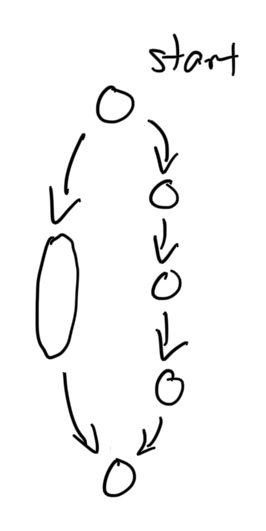
\includegraphics[width=3cm]{critical_path.jpeg}
\caption{Critical Path}
\label{fig:1}
\end{figure}
In general, it is assumed (from Amdahl's law) that optimizing the lines of code where a program spends most of its time will lead to the program running faster. 
Often, program performance is measured in latency but that is not always possible as not every program stops.
There are many applications where a program never stops running such as a web server.
Many programs today are multi-threaded, meaning that there are portions of code that can run in parallel. 
These portions of code may run for a long time, but speeding it up may not necessarily provide a performance increase. 
Every portion of a program (other than the start) is causally dependent on its predecessors.
The longest of these paths is called the critical path as no amount of parallelization can speed it up.
In \ref{fig:1}, we can see that the longest portion would be the block on the left, and it alone takes more CPU time than any other block.
However, a speedup of that block would provide no benefit. 
The chain of blocks on the right side is the critical path.
No matter how many processors we throw at this program, it is only as fast as the path on the right as that path is not parallelizable.

To build a tool to help identify what part of a program to optimize, we need to know how much of a performance boost we would get from speeding up each portion of code.
It is infeasible to speedup every portion of code automatically to do this, so we take advantage of the causal relationship between each piece of code and slow them down.
The overall slowdown caused by slowing down a particular piece of code is equivalent to the overall speedup you would receive from speeding up that piece of code. 
Coz, a causal profiler, finds potential speedups by experimenting on every part of the code and performing slowdowns. 
To speedup a particular portion, you can set progress points to let Coz know what to focus on. 
During experimentation, it was discovered that certain "speedups" would actually cause slow downs. 
That is, speeding up a portion of the code would actually result in the overall program being slower.
This can be caused by having congestion on a lock, disk, or network.


\end{document}
